
%(BEGIN_QUESTION)
% Copyright 2011, Tony R. Kuphaldt, released under the Creative Commons Attribution License (v 1.0)
% This means you may do almost anything with this work of mine, so long as you give me proper credit

Explain how the two control valves PV-33a and PV-33b work in conjunction with one another to control the overhead pressure inside the fractionation tower:

$$\includegraphics[width=15.5cm]{i0001rx01.eps}$$

Do you suppose these two control valves are split-ranged {\it progressively}, {\it exclusively}, or {\it complementarily}?

\vskip 20pt \vbox{\hrule \hbox{\strut \vrule{} {\bf Suggestions for Socratic discussion} \vrule} \hrule}

\begin{itemize}
\item{} A good problem-solving technique to apply in cases where we need to determine the direction of a change is to consider {\it limiting cases}.  Instead of asking ourselves what would happen if the fractionator overhead pressure changes slightly, we ask ourselves what would happen if the pressure changes {\it dramatically}.  Explain how this problem-solving technique applies to this particular system where we must analyze the split-ranged sequence of multiple valves.
\item{} Is the controller PC-33 direct or reverse acting?  Is this possible to tell from the given information, or must we know more in order to make this determination?
\item{} During typical unit operation, do you suppose PV-33a will be fully shut, wide open, or throttling?  Explain why.
\item{} During typical unit operation, do you suppose PV-33b will be fully shut, wide open, or throttling?  Explain why. 
\end{itemize}

\underbar{file i03569}
%(END_QUESTION)





%(BEGIN_ANSWER)

These two control valves are {\it progressively} split-ranged.  PV-33a is the first to open as the control signal pressure falls below 15 PSI, sending more cooling water to the overhead condenser E-8 (more cooling causes the vapors to condense at a faster rate, reducing pressure in the fractionation tower).  If a wide-open PV-33a is not enough to bring the tower pressure down to setpoint, valve PV-33b begins to open, venting vapor to the low-pressure flare where it may be safely burned off.

%(END_ANSWER)





%(BEGIN_NOTES)

What we have is this type of split-ranging:

$$\includegraphics[width=15.5cm]{i03569x01.eps}$$













\vskip 20pt \vbox{\hrule \hbox{\strut \vrule{} {\bf Virtual Troubleshooting} \vrule} \hrule}

This question is a good candidate for a ``Virtual Troubleshooting'' exercise.  Presenting the diagram to students, you first imagine in your own mind a particular fault in the system.  Then, you present one or more symptoms of that fault (something noticeable by an operator or other user of the system).  Students then propose various diagnostic tests to perform on this system to identify the nature and location of the fault, as though they were technicians trying to troubleshoot the problem.  Your job is to tell them what the result(s) would be for each of the proposed diagnostic tests, documenting those results where all the students can see.

During and after the exercise, it is good to ask students follow-up questions such as:

\begin{itemize}
\item{} What does the result of the last diagnostic test tell you about the fault?
\item{} Suppose the results of the last diagnostic test were different.  What then would that result tell you about the fault?
\item{} Is the last diagnostic test the best one we could do?
\item{} What would be the ideal order of tests, to diagnose the problem in as few steps as possible?
\end{itemize}

%INDEX% Final Control Elements, valve: split ranging
%INDEX% Process: distillation, generic (realistic P&ID shown)

%(END_NOTES)

